
\documentclass{article}

\usepackage[utf8]{inputenc}

\usepackage{amsmath}
\usepackage{graphicx}
\usepackage{amssymb}
\usepackage{float}

\setlength{\parskip}{\baselineskip}%
\setlength{\parindent}{0pt}%

\begin{document}

\title{Extended Coursework Report}
\author{lwp26}
\date{Feburary 2023}
\maketitle

\begin{abstract}
    \centering
    % Optimisation of tuned dampers to reduce the amplitude of resonant responses of a 3 degree of freedom structure
    In this report a model structure with 3 degrees of freedom will be hamonically excited to determine the resonant frequencies and mode shapes of the structure.
    The resonant frequnencies and mode shapes will be used to determine optimal design parameters for three seperate absorbers to reduce the resonant responses at each mode shape.
    % The optimal design parameters will be determined by using a genetic algorithm to minimise the resonant response of the structure.
    This approach can be used on real structures to reduce the amplitude of their resonant response to earthquakes.
\end{abstract}

\section{Introduction}

% Aims, Objectives and context
% context

Modern structures are designed to withstand a range of distributed static loads however they are vulnerable to harmonic excitations such as earthquakes.
The response of a structure to a harmonic excitation is determined by the resonant frequencies and mode shapes of the structure.

\subsection{Aims}

\begin{itemize}
\item To numerically model a 3 degree of freedom structure with 3 seperate absorbers to reduce the amplitude of the structure's resonant response to harmonic excitations represting earthquakes.
\item To
\end{itemize}

\section{Methodology}

% Summary of theory and information to reproduce

\section{Results}

\begin{figure}[H]
    \centering
    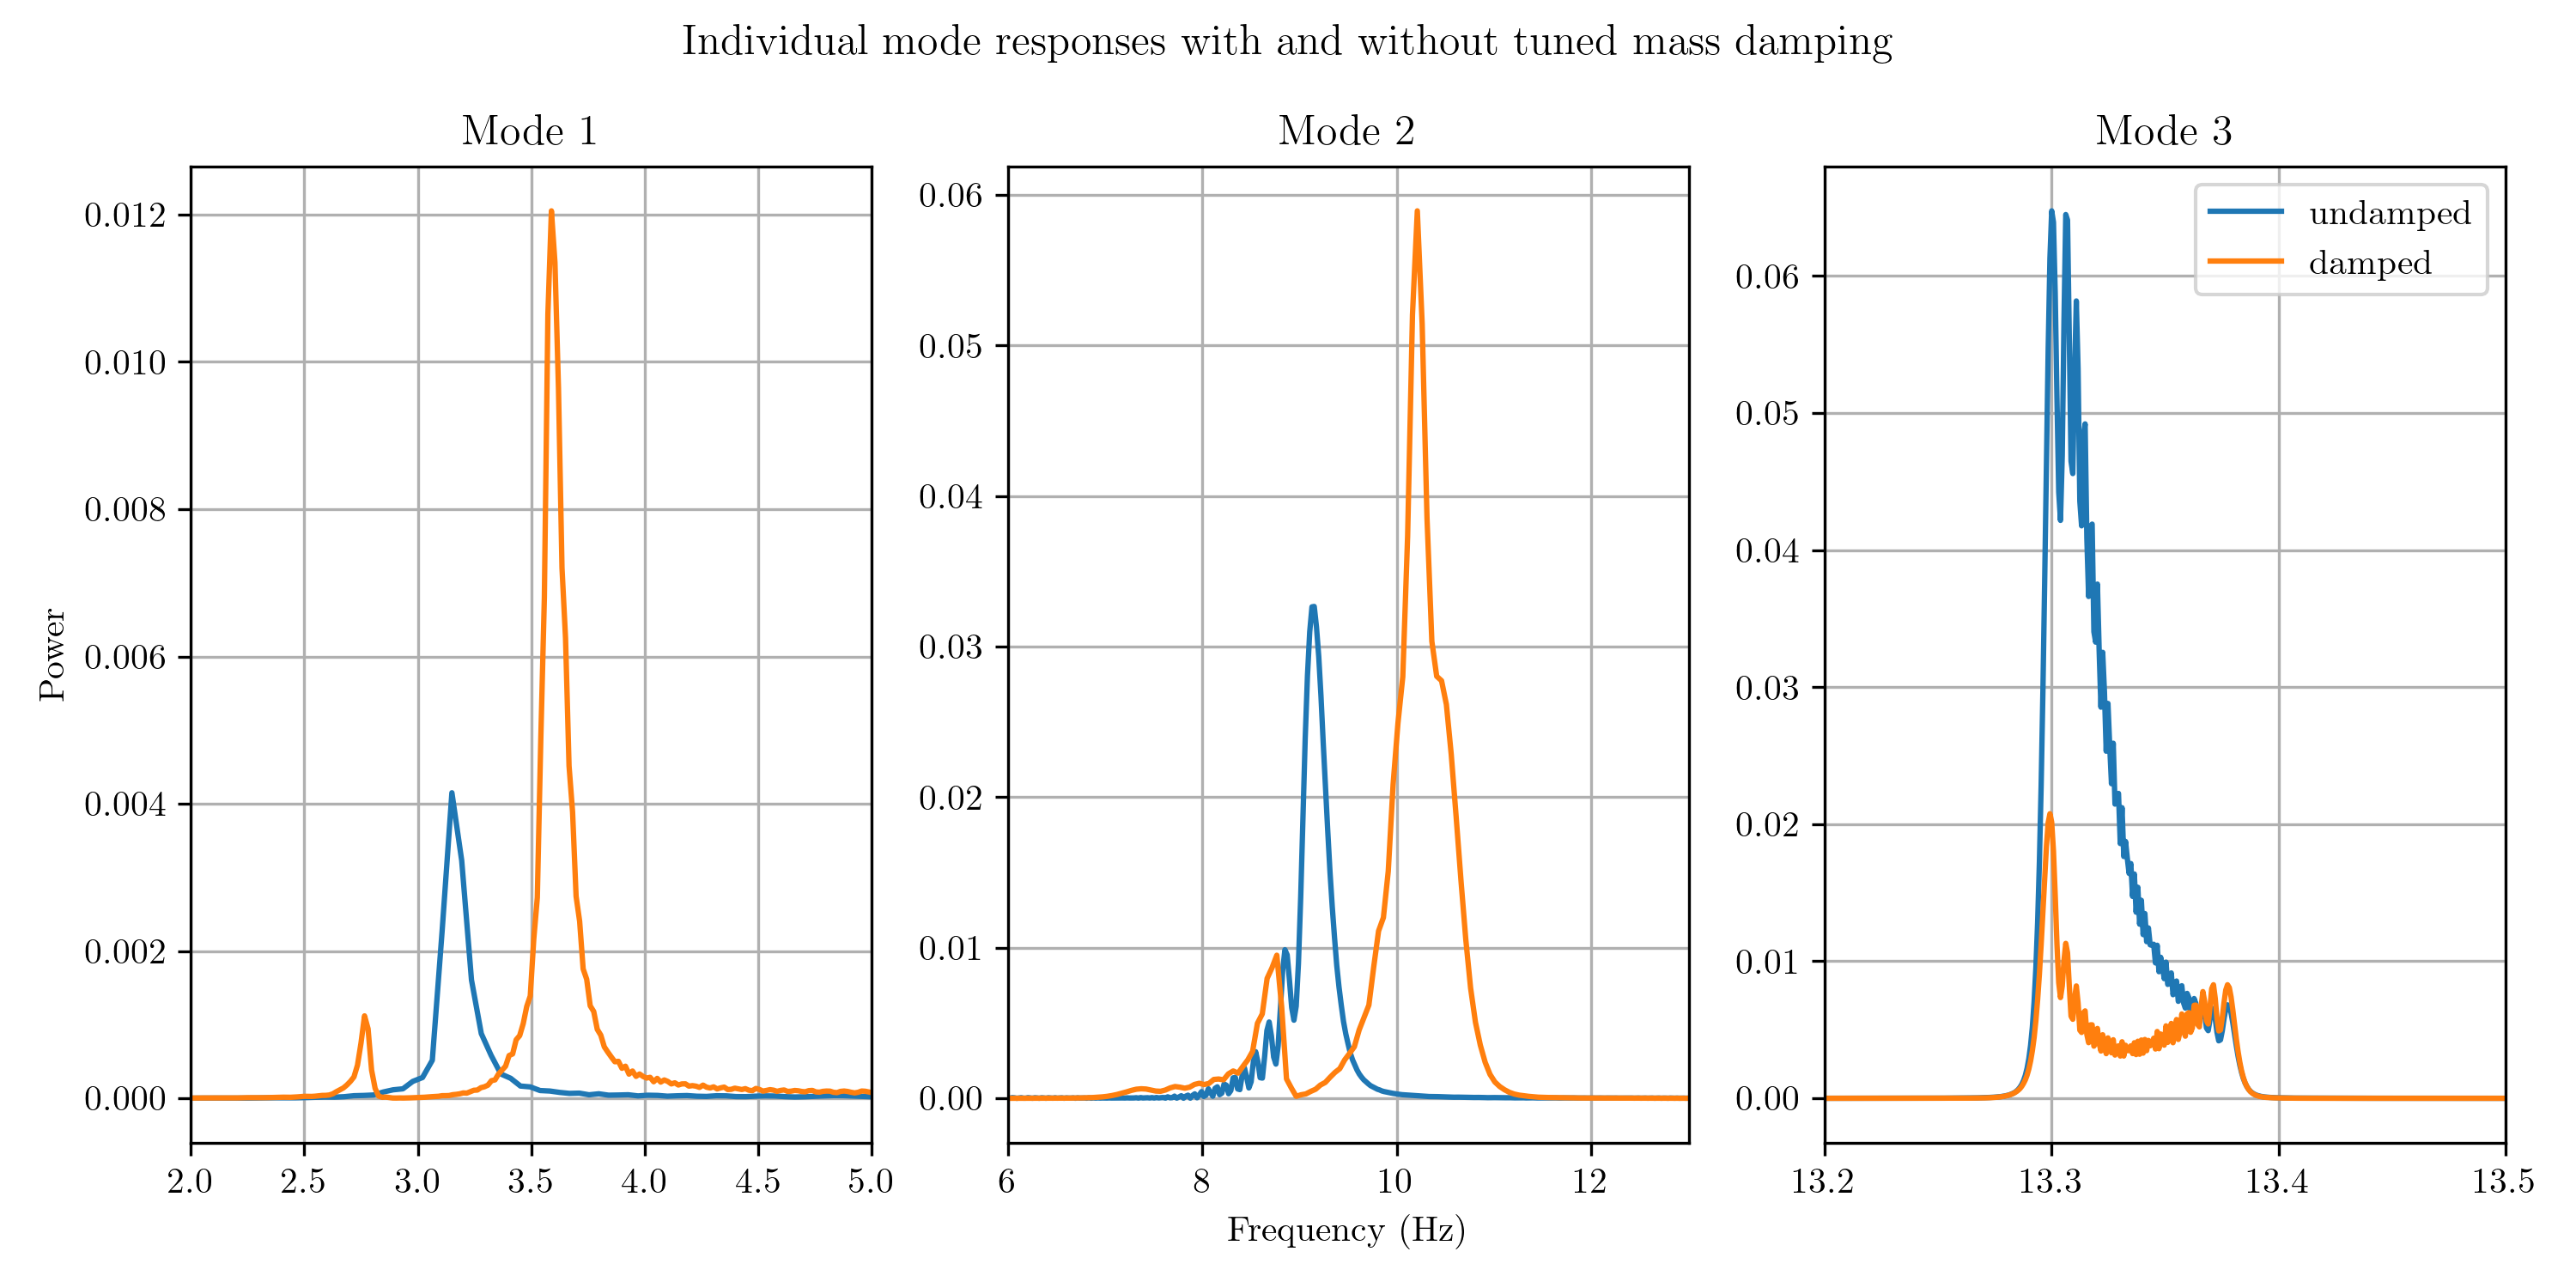
\includegraphics[width=1\textwidth]{modes.png}
    \caption{\label{fig:modes} Harmonic responses of each node before and after the addition of a single tuned damper to that node}
\end{figure}

\begin{figure}[H]
    \centering
    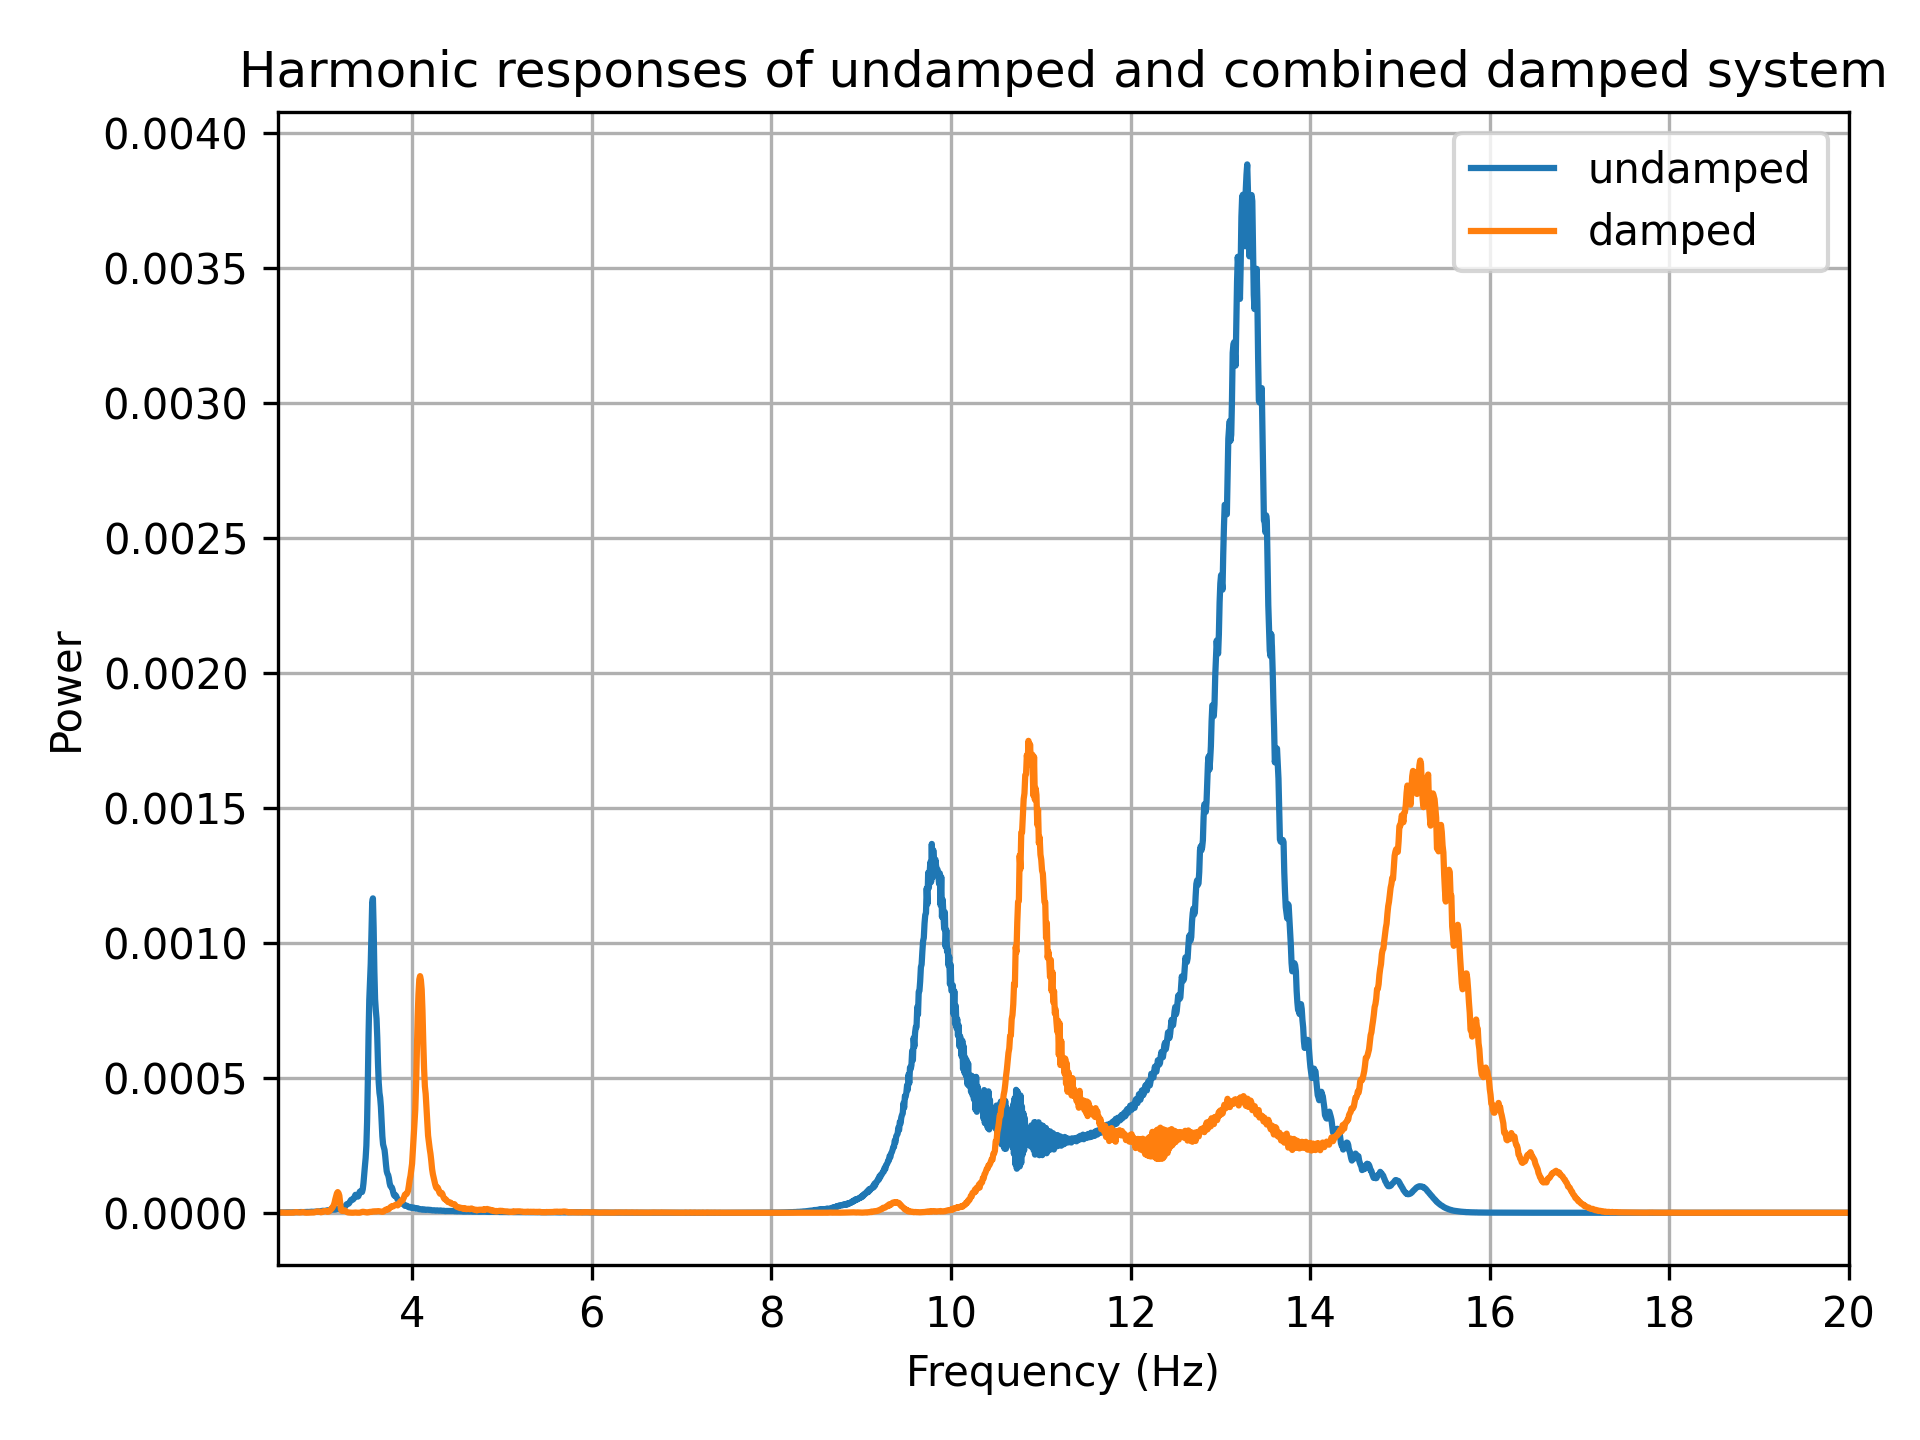
\includegraphics[width=1\textwidth]{combined_full_sweep.png}
    \caption{\label{fig:combined_full_sweep} Harmonic response of structure before and after the addition of 3 tuned dampers}
\end{figure}

\section{Discussion}

%interpret results and comment on anomalies

\section{Conclusion}

\end{document}